\documentclass[10pt,a4paper,oneside]{article}
\usepackage[brazil]{babel}
\usepackage[utf8]{inputenc}
\usepackage{amsmath}
\usepackage{amsfonts}
\usepackage{amssymb}
\usepackage[left=3cm,right=3cm,top=2cm,bottom=2cm]{geometry}

% Floats.
\usepackage{placeins}

\usepackage{xspace}
\usepackage{graphicx}

\newcommand{\arat}{Aratibutantã\xspace}
\newcommand{\baep}{Baependinha\xspace}
\newcommand{\itam}{Itamaracanã\xspace}
\newcommand{\jaqu}{Jaquereçaba\xspace}
\newcommand{\para}{Paranapitanga\xspace}

\newcommand{\adm}{Administração\xspace}
\newcommand{\comp}{Computação e Matemática\xspace}
\newcommand{\edu}{Educacional\xspace}
\newcommand{\eng}{Engenharia e Produção\xspace}
\newcommand{\hum}{Humanidades\xspace}
\newcommand{\jur}{Jurídica e Contábil\xspace}

% Tabelas.
\usepackage{booktabs}
\newcommand{\specialcell}[3][c]
{\begin{tabular}[#1]{@{}#2@{}}#3\end{tabular}}

\author{%
	Alexis A. Huf, %
	Alyson Pereira, %
	Bruno C. N. Oliveira,\\%
	Eliza Gomes, %
	Pedro H. Penna
	}

\title{Lista de Exercício I - Grupo 6}


\begin{document}

\maketitle

\paragraph{Questão 01}

A Tabela \ref{table: dados perdidos} apresenta a quantidade de dados perdidos (aqueles que não puderam ser recuperados por não estarem preenchidos) e seus respectivos percentuais em relação a cada variável analisada na base de dados em estudo. Foi observado um total de 106 dados perdidos para todas as variáveis, o que representa apenas $2.12\%$ do total. Pode-se considerar, portanto, como aceitável, uma vez que está abaixo dos $5\%$ definidos como percentual aceitável de dados perdidos.

\begin{table}[h]
\centering
\caption{Dados perdidos na base de dados.}
\label{table: dados perdidos}
\vspace{0.5em}
\begin{tabular}{c c c c c c}
	\toprule
	\textbf{Região} & \textbf{Área} & \textbf{Pagamento} & \textbf{Opinião} & \textbf{Renda} & \textbf{Idade} \\
	\midrule
	21 $(0.42\%)$   & 21 $(0.42\%)$ & 18 $(0.36\%)$      & 19 $(0.38\%)$    & 14 $(0.28\%)$  & 13 $(0.26\%)$ \\
	\bottomrule
\end{tabular}
\end{table}

%
% Dúvidas:
%   Devemos detalhar quis os erros (ex: Arábia, Araba)?
%
\paragraph{Questão 02}

A Tabela \ref{table: dados errados} resume os erros de coleta e seus respectivos percentuais na base de dados em estudo. Além de ausência de informação (conforme já mencionado na \textbf{Questão 01}), foram evidenciados erros de ortografia, digitação e formatação (ex: espaços em branco excedentes). 

As Tabelas \ref{table: erros-regiao}, \ref{table: erros-area}, \ref{table: erros-pagamento} e \ref{table: erros-opiniao} apresentam os erros observados para as variáveis qualitativas \textit{Região}, \textit{Área}, \textit{Pagamento} e \textit{Opinião}, respectivamente.
Para as variáveis quantitativas \textit{Renda} e \textit{Idade}, não foram observados erros na base de dados, isto é, valores infactíveis (ex: \textit{Renda} não positiva e \textit{Idade} inferior a 17 ou superior a 100 anos).

Para evitar que erros de ortografia e formatação sejam cometidos nas variáveis qualitativas, pode-se utilizar um formulário de múltipla escolha de modo a evitar que as informações sejam preenchidas de maneira textual. Já para as variáveis quantitativas, no caso de um formulário eletrônico, limites inferiores e superiores de valores válidos poderiam ser checado previamente à submissão da observação. Por outro lado, quanto aos dados perdidos que não foram preenchidos, é possível criar opções de modo que as pessoas possam informar explicitamente se não sabem ou, ainda, se não desejam responder. Desse modo, nenhuma informação seria ficaria perdida ou sem preenchimento. Ademais, é possível também aplicar um teste do questionário a um grupo menor de pessoas com o objetivo de testá-lo e verificar a sua adequação, para, posteriormente, aplicá-lo a um grupo maior. Assim, problemas de entendimento podem ser resolvidos nesta fase de teste, tendendo a reduzir o percentual de erros ou informações faltantes.

\begin{table}[!h]
\centering
\caption{Erros na base de dados.}
\vspace{0.5em}
\label{table: dados errados}
\begin{tabular}{c c c c c c}
	\toprule
	\textbf{Região} & \textbf{Área}  & \textbf{Pagamento} & \textbf{Opinião} & \textbf{Renda} & \textbf{Idade} \\
	\midrule
	135 $(2.71\%)$  & 114 $(2.28\%)$ & 132 $(2.64\%)$     & 123 $(2.46\%)$   & 0 $(0.00\%)$   & 0 $(0.00\%)$ \\
	\bottomrule
\end{tabular}
\end{table}

\begin{table}[!h]
\centering
\begin{minipage}[t]{0.49\textwidth}
\caption{Erros para a variável \textit{Região}.}
\vspace{0.5em}
\label{table: erros-regiao}
\begin{tabular}{l r r}
	\toprule
	\textbf{Erro} & \textbf{Absoluto}  & \textbf{Percentual} \\
	\midrule
	Arati      & 6  & $0.12\%$ \\
	Aratib     & 12 & $0.24\%$ \\
	Aratibu    & 5  & $0.10\%$ \\
	Aratibut   & 12 & $0.24\%$ \\
	Baepe      & 17 & $0.34\%$ \\
	Baepen     & 18 & $0.36\%$ \\
	Baepend    & 12 & $0.24\%$ \\
	Baependi   & 9  & $0.18\%$ \\
	Itama      & 5  & $0.10\%$ \\
	Itamar     & 6  & $0.12\%$ \\
	Itamara    & 3  & $0.06\%$ \\
	Itamarac   & 7  & $0.14\%$ \\
	Jaque      & 5  & $0.10\%$ \\
	Jaquer     & 10 & $0.20\%$ \\
	Jaquere    & 5  & $0.10\%$ \\
	Jaquereç   & 3  & $0.06\%$ \\
	\midrule
	\textbf{Total de erros}  & 135  & $2.71\%$ \\	
	\bottomrule
\end{tabular}
\end{minipage}
%
\begin{minipage}[t]{0.49\textwidth}
\caption{Erros para a variável \textit{Área}.}
\vspace{0.5em}
\label{table: erros-area}
\begin{tabular}{l r r}
	\toprule
	\textbf{Erro} & \textbf{Absoluto}  & \textbf{Percentual} \\
	\midrule
	Admin      & 3   & $0.06\%$ \\
	Admini 	   & 3   & $0.06\%$ \\
	Adminis    & 2   & $0.04\%$ \\
	Administ   & 5   & $0.10\%$ \\
	Compu      & 1   & $0.02\%$ \\
	Comput     & 2   & $0.04\%$ \\
	Computa    & 2   & $0.04\%$ \\
	Computaç   & 1   & $0.02\%$ \\
	Educa      & 2   & $0.04\%$ \\
	Educac     & 2   & $0.04\%$ \\
	Educaci    & 1   & $0.02\%$ \\
	Educacio   & 1   & $0.02\%$ \\
	Engen      & 15  & $0.30\%$ \\
	Engenh     & 9   & $0.18\%$ \\
	Engenha    & 8   & $0.16\%$ \\
	Engenhar   & 14  & $0.28\%$ \\
	Human      & 3   & $0.06\%$ \\
	Humani     & 3   & $0.06\%$ \\
	Humanid    & 4   & $0.08\%$ \\
	Humanida   & 5   & $0.10\%$ \\
	Juríd      & 3   & $0.06\%$ \\
	Jurídi     & 7   & $0.14\%$ \\
	Jurídic    & 11  & $0.22\%$ \\
	Jurídica   & 7   & $0.14\%$ \\	
	\midrule
	\textbf{Total de erros}  & 114  & $2.28\%$ \\	
	\bottomrule
\end{tabular}
\end{minipage}
\end{table}

\begin{table}[!h]
\centering
\begin{minipage}[t]{0.49\textwidth}
\caption{Erros para a variável \textit{Pagamento}.}
\vspace{0.5em}
\label{table: erros-pagamento}
\begin{tabular}{l r r}
	\toprule
	\textbf{Erro} & \textbf{Absoluto}  & \textbf{Percentual} \\
	\midrule
	Auxíl     		& 3   & $0.06\%$ \\
	Auxíli 	  		& 2   & $0.04\%$ \\
	Auxílio    	 	& 2   & $0.04\%$ \\
	Auxílio \textit{(espaço)}   	& 1   & $0.02\%$ \\
	Bolsa      	 	& 3   & $0.06\%$ \\
	Bolsas     	 	& 1   & $0.02\%$ \\
	Bolsas d   	 	& 5   & $0.10\%$ \\
	Finan      	 	& 15  & $0.30\%$ \\
	Financ     	 	& 13  & $0.26\%$ \\
	Financi    	 	& 19  & $0.38\%$ \\
	Financia   	 	& 13  & $0.26\%$ \\
	Incen      	 	& 8   & $0.16\%$ \\
	Incent     	 	& 11  & $0.22\%$ \\
	Incenti    	 	& 11  & $0.22\%$ \\
	Incentiv   	 	& 10  & $0.20\%$ \\
	Recur      	 	& 4   & $0.08\%$ \\
	Recurs     	 	& 4   & $0.08\%$ \\
	Recurso    	 	& 5   & $0.10\%$ \\
	Recursos   	 	& 2   & $0.04\%$ \\	
	\midrule
	\textbf{Total de erros}  & 132  & $2.64\%$ \\	
	\bottomrule
\end{tabular}
\end{minipage}
%
\begin{minipage}[t]{0.49\textwidth}
\caption{Erros para a variável \textit{Opinião}.}
\vspace{0.5em}
\label{table: erros-opiniao}
\begin{tabular}{l r r}
	\toprule
	\textbf{Erro} & \textbf{Absoluto}  & \textbf{Percentual} \\
	\midrule
	Indifer    & 14  & $0.28\%$ \\
	Indifere   & 16  & $0.32\%$ \\
	Insatis    & 7   & $0.14\%$ \\
	Insatisf   & 10  & $0.20\%$ \\
	Muito i    & 3   & $0.06\%$ \\
	Muito in   & 5   & $0.10\%$ \\
	Muito s    & 22  & $0.44\%$ \\
	Muito sa   & 28  & $0.56\%$ \\
	Satisfe    & 10  & $0.20\%$ \\
	Satisfei   & 8   & $0.16\%$ \\	
	\midrule
	\textbf{Total de erros}  & 123  & $2.46\%$ \\	
	\bottomrule
\end{tabular}
\end{minipage}
\end{table}


\begin{table}[!h]
\centering

\end{table}

\FloatBarrier

\paragraph{Questão 03}

A tabela de frequências para a variável \textit{Região} está indicada na Tabela \ref{table: tabela frequencias regiao}. Por análise, pode-se observar que a região predominante na base dados é \textit{\baep}, embora não represente a maioria absoluta.

\begin{table}[!h]
\centering
\caption{Frequências para a variável \textit{Região}.}
\vspace{0.5em}
\label{table: tabela frequencias regiao}
\vspace{0.5em}
\begin{tabular}{c c c c c}
	\toprule
	\textbf{\arat}    & \textbf{\baep}   & \textbf{\itam}  & \textbf{\jaqu}  & \textbf{\para} \\
	\midrule
	1185 $(23.80\%)$  & 2294 $(46.07\%)$ & 843 $(16.93\%)$ & 536 $(10.77\%)$ & 121 $(2.43\%)$ \\
	\bottomrule
\end{tabular}
\end{table}

\paragraph{Questão 04}

A tabela de frequências para a variável \textit{Área} está indicada na Tabela \ref{table: tabela frequencias area}. Por análise, pode-se observar que a \textit{Área} predominante da \texttt{TYU} modificou-se para \eng.


\begin{table}[h]
\centering
\caption{Frequências para a variável \textit{Área}.}
\vspace{0.5em}
\label{table: tabela frequencias area}
\vspace{0.5em}
\begin{tabular}{c c c c c c}
	\toprule
	\textbf{\adm}   & \textbf{\comp} & \textbf{\edu} & \textbf{\eng}    & \textbf{\hum}   & \textbf{\jur} \\
	\midrule
	592 $(11.89\%)$ & 296 $(5.94\%)$ & 338 $(6.79\%)$ & 1741 $(34.97\%)$ & 503 $(10.10\%)$ & 1509 $(30.31\%)$ \\
	\bottomrule
\end{tabular}
\end{table}


\paragraph{Questão 05}

A tabela de frequências para a variável \textit{Pagamento} está indicada na Tabela \ref{table:frequencias-pagamento}. Por análise, pode-se observar que os recursos usados para pagar as mensalidades do curso são oriundos, em sua maioria, de \textit{Financiamento Bancário} representando $43.98\%$. Já o pagamento  oriundo de \textit{Incentivos Federais} apresenta-se como o segundo mais utilizado, com  $29.06\%$.  Portanto, a maior dependência de pagamento está no \textit{Financiamento Bancário}, embora  \textit{Incentivos Federais} representem a segunda forma de pagamento mais utilizada.

\begin{table}[!h]
\centering
\caption{Frequências para a variável \textit{Pagamento}.}
\vspace{0.5em}
\label{table:frequencias-pagamento}
\begin{tabular}{c c c c c}
	\toprule
	\textbf{Aux. de Fam.}    & \textbf{Bolsas}   & \textbf{Financ. Banc.}  & \textbf{Inc. Federais} & \textbf{Rec. Próprios} \\
	\midrule
	257 $(5.16\%)$ & 328 $(6.58\%)$ & 2191 $(43.98\%)$ & 1448 $(29.06\%)$ & 758 $(15.21\%)$ \\
	\bottomrule
\end{tabular}
\end{table}

\paragraph{Questão 06}

A tabela de frequências para a variável \textit{Opinião} está indicada na Tabela \ref{table:frequencias-opiniao}. Por análise, pode-se observar que a opinião predominante na base dados é \textit{Muito satisfeito}. O grupo dos que mencionaram estarem \textit{Muito satisfeito} e \textit{Satisfeito} totaliza $55,29\%$. Podemos considerar, portanto, que a maioria dos alunos da TYU que opinaram estão satisfeitos com a EAD.

\begin{table}[!h]
\centering
\caption{Frequências para a variável \textit{Opinião}.}
\vspace{0.5em}
\label{table:frequencias-opiniao}
\begin{tabular}{c c c c c}
	\toprule
	\textbf{Indiferente}    & \textbf{Insatisfeito}   & \textbf{Muito insatisfeito}  & \textbf{Muito satisfeito} & \textbf{Satisfeito} \\
	\midrule
	1006 $(20.20\%)$ & 749 $(15.04\%)$ & 472 $(9.48\%)$ & 1719 $(34.51\%)$ & 1035 $(20.78\%)$ \\
	\bottomrule
\end{tabular}
\end{table}


\paragraph{Questão 07}

A tabela \ref{table:medidas-renda} foi construída com base nos valores de \textit{Renda} disponíveis na base de dados e apresenta as diversas medidas calculadas para análise desta variável. Vale observar que, para fins de análise, criou-se uma nova variável com base na renda multiplicando-a por 880 (valor utilizado para o salário mínimo). Pode-se observar que pelo menos três quartos dos alunos de EAD da TYU ainda mantém renda familiar inferior a $R\$2450,00$, uma vez que o quartil superior da base de dados para essa variável é de $R\$2402,40$.

Por meio da Curtose, é possível analisar também o grau de achatamento da distribuição como sendo leptocúrtica - uma curva de frequência mais aguda. Além disso, como a média e mediana são diferentes, existe uma assimetria de $9.94$, isto é, a distribuição dos dados é assimétrica à direita ou positiva. Pode-se interpretar, ademais, a dispersão de $76\%$ dos dados em relação à média, com base no Coeficiente de variação.
Com relação aos valores discrepantes, observa-se que o conjunto de dados analisados e disponíveis na base de dados contempla $296$ valores de renda acima de $4224.00$. Um histograma da variável idade é apresentado na Figura \ref{fig:histograma-renda}.

\begin{table}[!h]
\centering
\caption{Análise das medidas para a variável variável \textit{Renda}}
\vspace{0.5em}
\label{table:medidas-renda}
\begin{tabular}{l r}
	\toprule
	\textbf{Medida}               & \textbf{Valor} \\
	\midrule
	Média                         &  $2056,05$     \\
	Moda                          &  $906,40$      \\
	Mediana                       &  $1628,00$     \\
	Variância                     &  $2449929,23$  \\
	Desvio Padrão                 &  $1565.38$     \\
	Coeficiente de Variação       &  $76\%$        \\
	Assimetria                    &  $9.94$        \\
	Curtose                       &  $253.91$      \\
	Mínimo                        &  $880.00$      \\
	Máximo                        &  $53504.00$    \\
	Quartil Inferior (Qi)         &  $1188.00$     \\
	Quartil Superior (Qs)         &  $2402.40$     \\
	Diferença Interquartil        &  $1214.40$     \\
	$Qi-1.5x(Qs-Qi)$ (Discrep. -) &  $-633.60$     \\
	$Qs+1.5x(Qs-Qi)$ (Discrep. +) &  $4224.00$     \\
	Dados Totais                  &  $5000$        \\
	Dados Válidos                 &  $4986$        \\
	Dados Perdidos                &  $14$          \\
	Dados Discrepantes            &  $296$         \\
	\bottomrule
\end{tabular}
\end{table}

\begin{figure}[!h]
	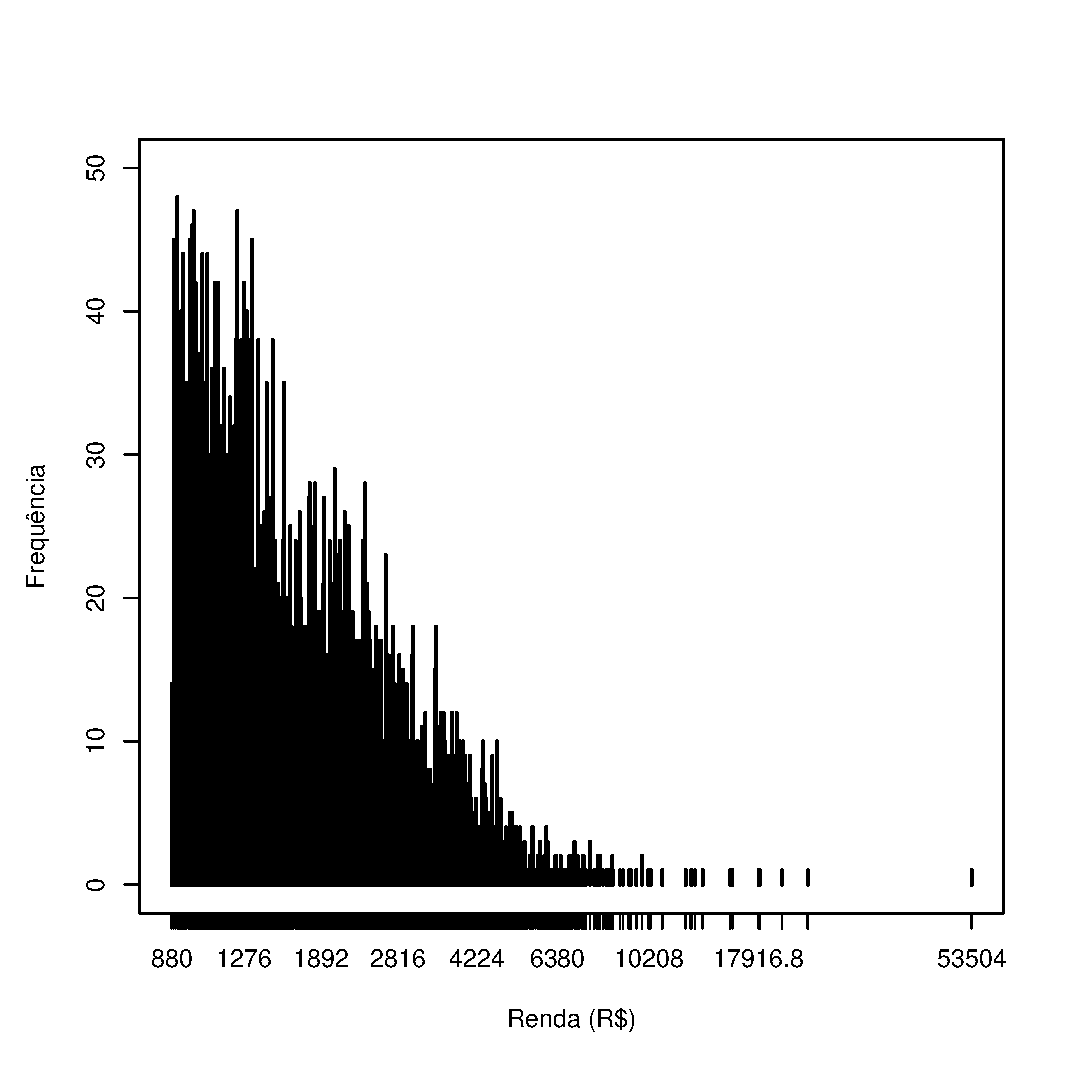
\includegraphics[width=\linewidth]{plots/histogram_renda_log.eps}
	\caption{Histograma da varável \textit{Renda}. Escala logarítimica no eixo $x$}
	\label{fig:histograma-renda}
\end{figure}

%
% {GRÁFICOS}
%

\FloatBarrier

\paragraph{Questão 08}



\begin{table}[!h]
	\centering
	\caption{Análise das medidas para a variável variável \textit{idade}}
	\vspace{0.5em}
	\label{table:medidas-idade}
	\begin{tabular}{l r}
		\toprule
		\textbf{Medida}               & \textbf{Valor} \\
		\midrule
		Média                         &  $32.18$ \\
		Moda                          &  $32.00$ \\
		Mediana                       &  $32$ \\
		Variância                     &  $31.83$ \\
		Desvio Padrão                 &  $5.64$ \\
		Coeficiente de Variação       &  $18 \%$ \\
		Assimetria                    &  $1.205$ \\
		Curtose                       &  $6.19$ \\
		Mínimo                        &  $18$ \\
		Máximo                        &  $70$ \\
		Quartil Inferior (Qi)         &  $29$ \\
		Quartil Superior (Qs)         &  $35$ \\
		Diferença Interquartil        &  $6$ \\
		$Qi-1.5x(Qs-Qi)$ (Discrep. -) &  $20$ \\
		$Qs+1.5x(Qs-Qi)$ (Discrep. +) &  $44$ \\
		Dados Totais                  &  $5000$ \\
		Dados Válidos                 &  $4987$ \\
		Dados Perdidos                &  $13$ \\
		Dados Discrepantes            &  $0$ \\
		\bottomrule
	\end{tabular}
\end{table}
\end{document}
